\begin{center}
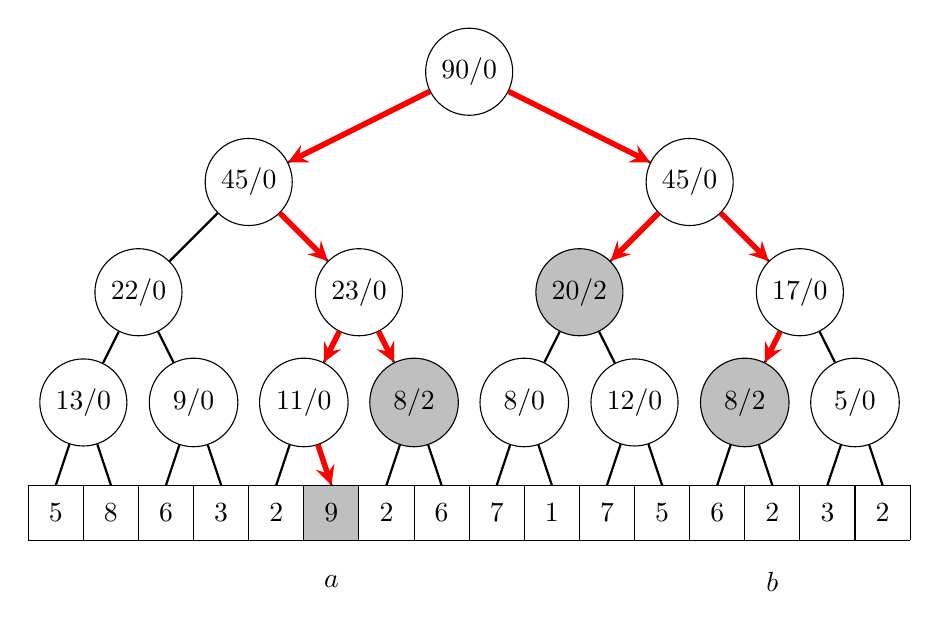
\begin{tikzpicture}[scale=0.7]
\fill[color=gray!50] (5,0) rectangle (6,1);
\draw (0,0) grid (16,1);

\foreach \x  [count=\pos from 0] in {5,8,6,3,2,9,2,6,7,1,7,5,6,2,3,2}{
  \pgfmathsetmacro{\posp}{\pos+0.5}
  \node[anchor=center] at (\posp, 0.5) {\x};
}

%\node[anchor=center] at (0.5, 0.5) {5};
%\node[anchor=center] at (1.5, 0.5) {8};
%\node[anchor=center] at (2.5, 0.5) {6};
%\node[anchor=center] at (3.5, 0.5) {3};
%\node[anchor=center] at (4.5, 0.5) {2};
%\node[anchor=center] at (5.5, 0.5) {9};
%\node[anchor=center] at (6.5, 0.5) {2};
%\node[anchor=center] at (7.5, 0.5) {6};
%\node[anchor=center] at (8.5, 0.5) {7};
%\node[anchor=center] at (9.5, 0.5) {1};
%\node[anchor=center] at (10.5, 0.5) {7};
%\node[anchor=center] at (11.5, 0.5) {5};
%\node[anchor=center] at (12.5, 0.5) {6};
%\node[anchor=center] at (13.5, 0.5) {2};
%\node[anchor=center] at (14.5, 0.5) {3};
%\node[anchor=center] at (15.5, 0.5) {2};
%
\node[draw, circle] (a) at (1,2.5) {13/0};
\path[draw,thick,-] (a) -- (0.5,1);
\path[draw,thick,-] (a) -- (1.5,1);
\node[draw, circle,minimum size=32pt] (b) at (3,2.5) {9/0};
\path[draw,thick,-] (b) -- (2.5,1);
\path[draw,thick,-] (b) -- (3.5,1);
\node[draw, circle,minimum size=32pt] (c) at (5,2.5) {11/0};
\path[draw,thick,-] (c) -- (4.5,1);
\path[draw,thick,-] (c) -- (5.5,1);
\node[draw, circle,fill=gray!50,minimum size=32pt] (d) at (7,2.5) {8/2};
\path[draw,thick,-] (d) -- (6.5,1);
\path[draw,thick,-] (d) -- (7.5,1);
\node[draw, circle,minimum size=32pt] (e) at (9,2.5) {8/0};
\path[draw,thick,-] (e) -- (8.5,1);
\path[draw,thick,-] (e) -- (9.5,1);
\node[draw, circle] (f) at (11,2.5) {12/0};
\path[draw,thick,-] (f) -- (10.5,1);
\path[draw,thick,-] (f) -- (11.5,1);
\node[draw, circle,fill=gray!50,minimum size=32pt] (g) at (13,2.5) {8/2};
\path[draw,thick,-] (g) -- (12.5,1);
\path[draw,thick,-] (g) -- (13.5,1);
\node[draw, circle,minimum size=32pt] (h) at (15,2.5) {5/0};
\path[draw,thick,-] (h) -- (14.5,1);
\path[draw,thick,-] (h) -- (15.5,1);
%
\node[draw, circle] (i) at (2,4.5) {22/0};
\path[draw,thick,-] (i) -- (a);
\path[draw,thick,-] (i) -- (b);
\node[draw, circle] (j) at (6,4.5) {23/0};
\path[draw,thick,-] (j) -- (c);
\path[draw,thick,-] (j) -- (d);
\node[draw, circle,fill=gray!50] (k) at (10,4.5) {20/2};
\path[draw,thick,-] (k) -- (e);
\path[draw,thick,-] (k) -- (f);
\node[draw, circle] (l) at (14,4.5) {17/0};
\path[draw,thick,-] (l) -- (g);
\path[draw,thick,-] (l) -- (h);
%
\node[draw, circle] (m) at (4,6.5) {45/0};
\path[draw,thick,-] (m) -- (i);
\path[draw,thick,-] (m) -- (j);
\node[draw, circle] (n) at (12,6.5) {45/0};
\path[draw,thick,-] (n) -- (k);
\path[draw,thick,-] (n) -- (l);
%
\node[draw, circle] (o) at (8,8.5) {90/0};
\path[draw,thick,-] (o) -- (m);
\path[draw,thick,-] (o) -- (n);
%
\path[draw=red,thick,-stealth,line width=2pt] (o) -- (m);
\path[draw=red,thick,-stealth,line width=2pt] (o) -- (n);
%
\path[draw=red,thick,-stealth,line width=2pt] (m) -- (j);
\path[draw=red,thick,-stealth,line width=2pt] (j) -- (c);
\path[draw=red,thick,-stealth,line width=2pt] (j) -- (d);
\path[draw=red,thick,-stealth,line width=2pt] (c) -- (5.5,1);
%
\path[draw=red,thick,-stealth,line width=2pt] (n) -- (k);
\path[draw=red,thick,-stealth,line width=2pt] (n) -- (l);
%
\path[draw=red,thick,-stealth,line width=2pt] (l) -- (g);
%
\node at (5.5,-0.75) {$a$};
\node at (13.5,-0.75) {$b$};

\end{tikzpicture}
\end{center}